\section{Performance Evaluation}
\label{sec:pe}
We consider a $5000 \times 5000 m^2$ sparse sensing field with
$100$ relay nodes.
The Poisson-contact
mobility model is quasi-synthetic,
in which the parameter $\lambda$ is set to $0.004$.
The source node is fixed at the center of the network scenario.
The speed of nodes is randomly selected in a uniform distribution
changing from 4 to 10 m/s,
and the communication range of these nodes is set to be $20$$m$.
The parameter $\alpha$ is limited,
i.e.,
$\alpha \in [0, 1]$.
We consider two cases in the simulations.
In the first case (Section~\ref{subsec:wo_detc}),
we set $U(t)=0$,
which means there is no selfish detection.
In the second case (Section~\ref{subsec:full_detc}),
we adopt the selfish detection method and keep detecting during whole lifetime of network.
In each simulation,
$M$ messages are created,
whose maximal lifetime $T_m$ increases from $0$$s$ to $2000$$s$.
Note that,
all statistical results of our scheme are obtained by
repeating 50 times.

\subsection{Accuracy Analysis Based on Simulations}
\label{subsec:pe_valid}
\begin{figure}
  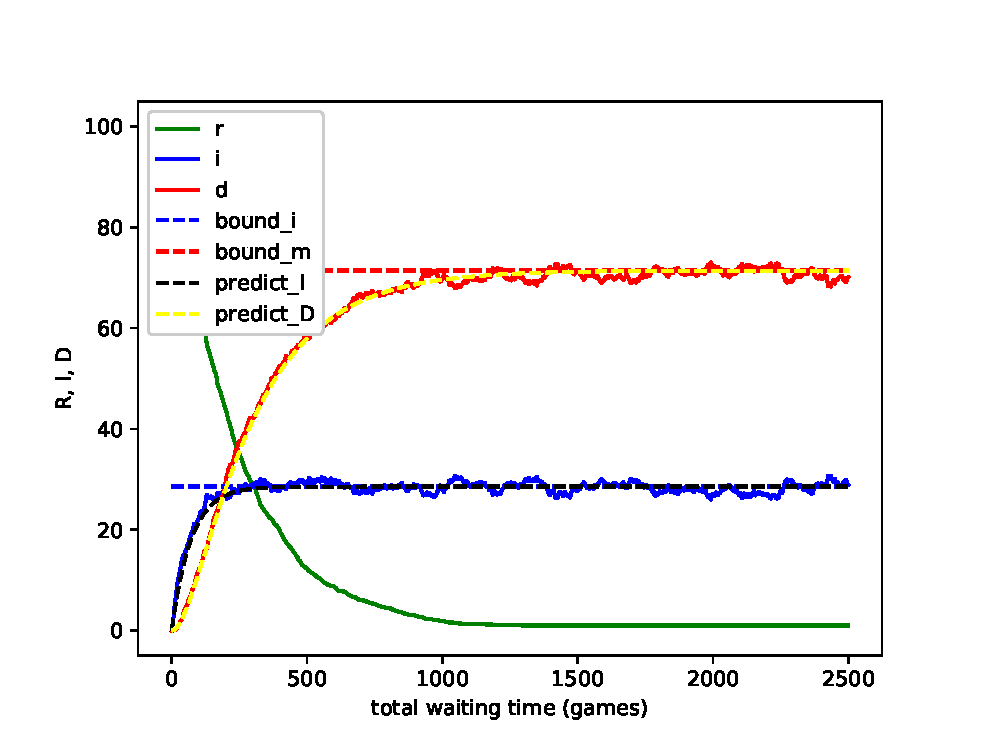
\includegraphics[width=.45\textwidth]{fig/twohop_without_detection.eps}
  \caption{Comparison of the theoretical and simulation results of the proposed ODE model in  case $1$.}
  \label{fig:twohop_predict_wod}
\end{figure}
As shown in Sections~\ref{sec:ode_model} and~\ref{sec:opt_detect},
we mathematically model the state transition of nodes by the ODEs,
based on which we analyze the optimal control through the Pontryagin's Maximum Principle.
It is critical to verity the accurate of the proposed model.
Therefore,
in the first experiment,
we compare the the simulation and the analytical results to check the accuracy of models.
Fig.~\ref{fig:twohop_predict_wod} shows
the comparison between the simulation and the analytical result in Case $1$,
in which $D(t)$, $I(t)$ and $R(t)$ with time $t$ are computed from prediction and simulations
when $\lambda = 0.004$, $\rho = 0.01$, $N=100$ and $T=2,500$,
and the dotted lines represent the analytical results.
As can be seen,
the analytical results match the simulation results reasonably,
which validates the proposed analytical model.

The result in Fig.~\ref{fig:twohop_predict_full_d} shows that
the accuracy of the proposed ODE models in Case $2$.
In this figure,
$I(t)$, $D(t)$ and $R(t)$ with time $t$  are computed from prediction and simulations
when $\lambda = 0.004$, $\rho = 0.011$, $N=100$, $T_{m} = 1$ and $T=2,500$.
According to Equation~(\ref{eq:IDR_full_solu}),
we can know that the analytical results about total number of $D(t)$ is in a monotone increasing
situation when the growing $T$.
The blue line in Fig.~\ref{fig:twohop_predict_full_d} proves this conclusion.
However, 
the number of selfish number reduce to $20$ when comparing with Fig.~\ref{fig:twohop_predict_wod}.
This is because adopting detection methods will mitigate the selfish behaviour of nodes.
Fig~\ref{fig:twohop_predict_full_d} verifies the accuracy of the proposed ODE model again.

\subsection{Efficacy of the approximate method}
\begin{figure}
  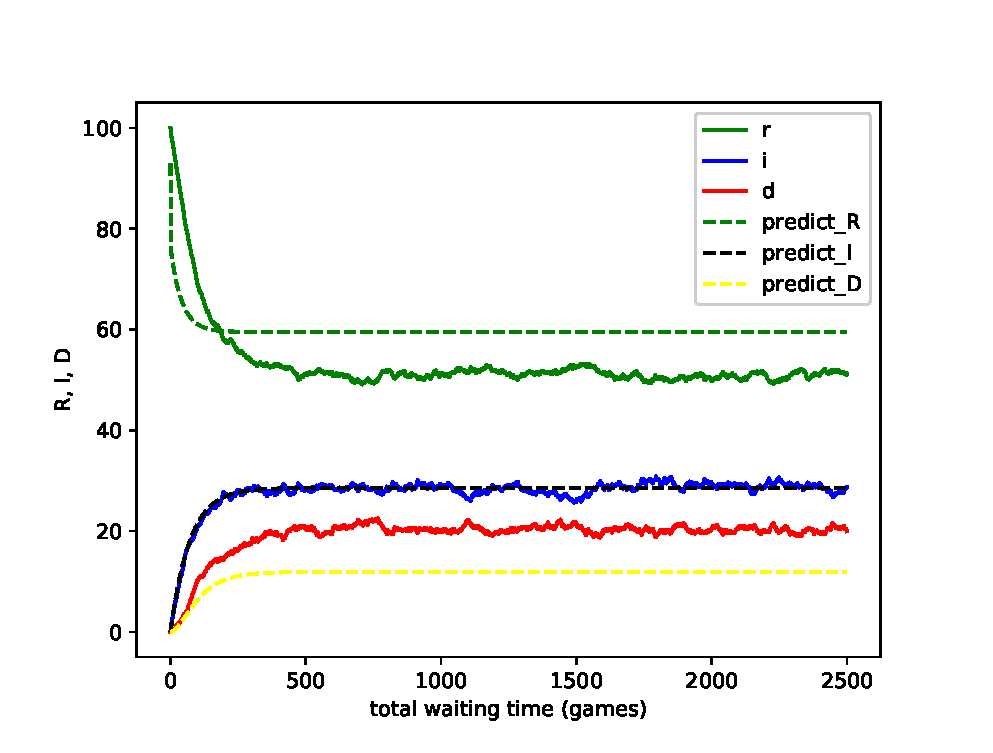
\includegraphics[width=.45\textwidth]{fig/twohop_with_fully_detection.eps}
  \caption{Comparison of the theoretical an simulation results or the proposed ODE model in case $2$.}
  \label{fig:twohop_predict_full_d}
\end{figure}
In the second experiment,
we analysis efficacy of the approximate method.
Fig.~\ref{fig:pe_opt_state_time} shows the state transition of nodes with time $T$,
in which $M(t)$ represent ,
$I(t)$ represent ,
$S(t)$ represent and $\lambda_2$ represent.
As we can see,
the value of $M(t)$ and the value of $\lambda_2$ decrease 
with $T$. 
In contrast,
both $S(t)$ and $I(t)$ have growing trend with increasing $T$.
This verify the sate transition is balanced.

Fig.~\ref{fig:pe_opt_control_Ut} shows the control variable $U(t)$ with increasing time.
From this figure, 
we can easily obtain the optimal control policy to
minimize the $J$. 
For example, 
when $T$ equals to $100$, 
the complete detection is open.
When time equals to $450$,
the network will switch from an `on state' to an `off state'.
\subsection{Optimal solution of selfish detection}
\begin{figure}
  \centering
  {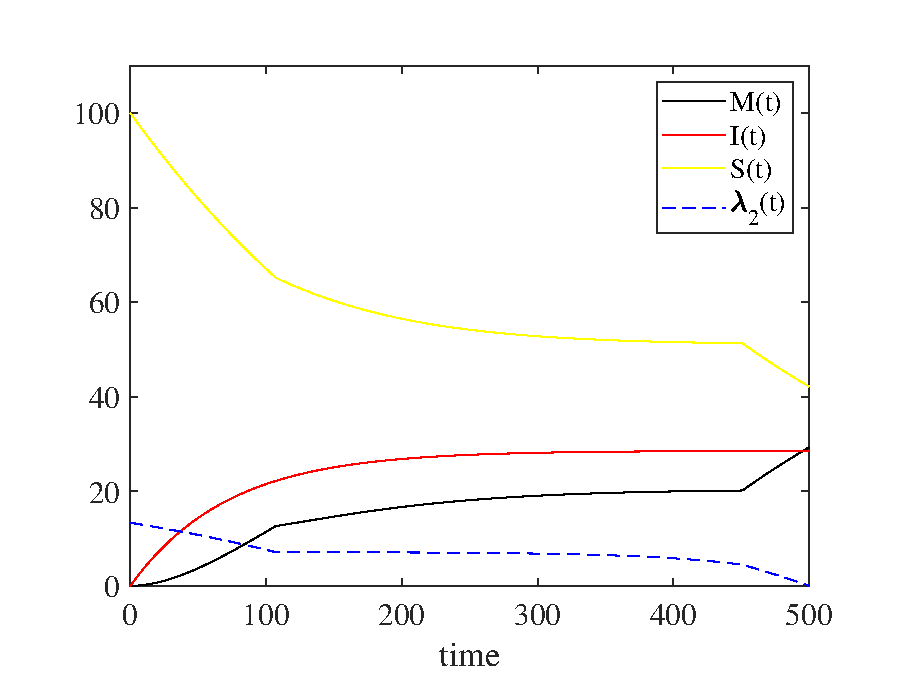
\includegraphics[width=0.47\textwidth]{fig/state.eps}}
     \caption{State variable of analysis with time.}
     \label{fig:pe_opt_state_time}
\end{figure}
\begin{figure}
  \centering
  {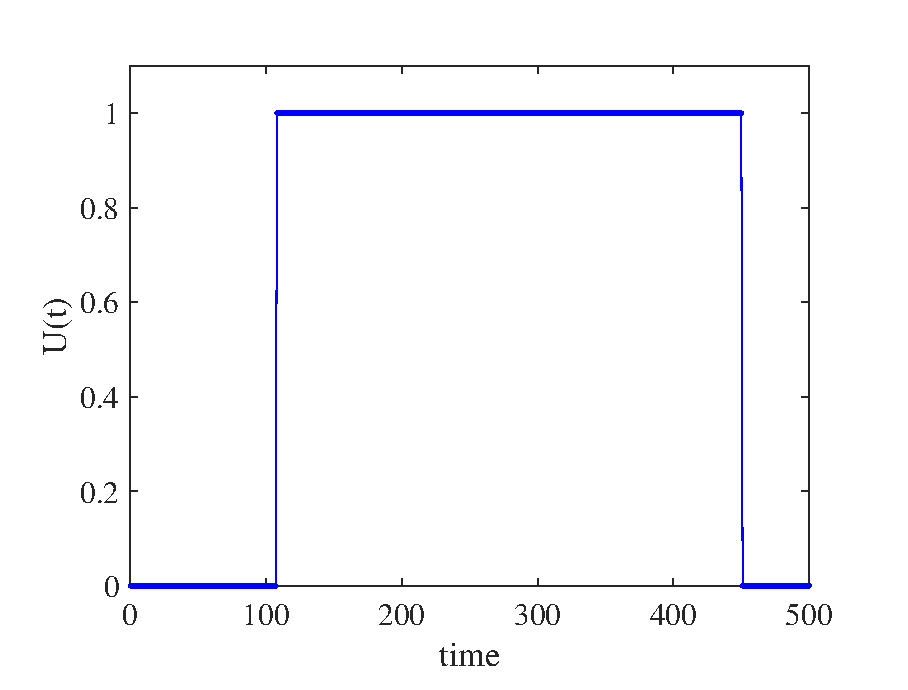
\includegraphics[width=0.47\textwidth]{fig/Ut.eps}}
     \caption{The optimal control policy of $U(t)$.}
     \label{fig:pe_opt_control_Ut}
\end{figure}
\begin{figure}
  \centering
  {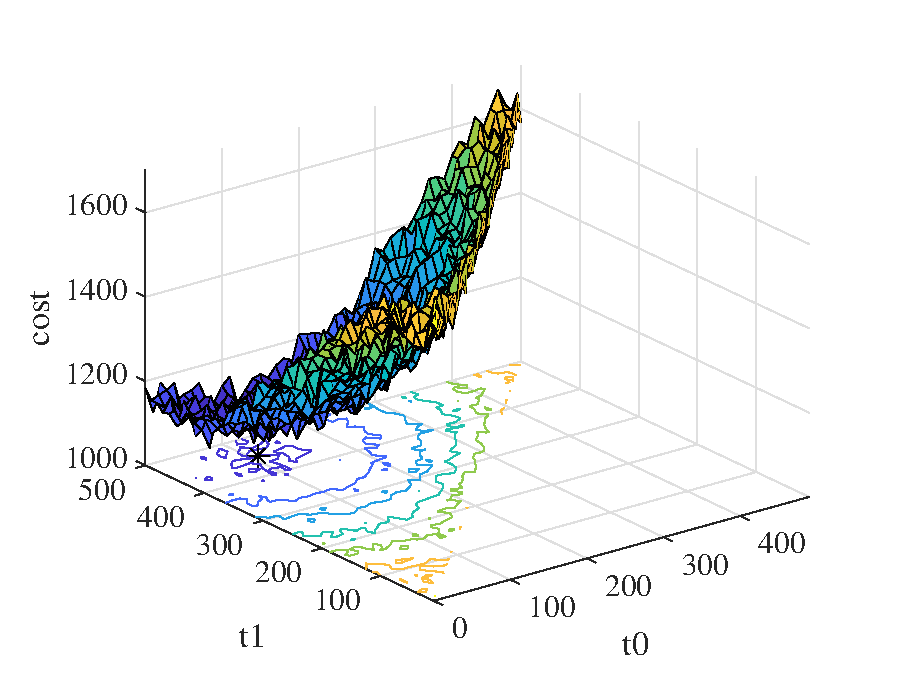
\includegraphics[width=0.47\textwidth]{fig/cost_all_t0t1.eps}}
     \caption{Different choices of $t0$ and $t1$.}
     \label{fig:pe_diff_choices}
\end{figure}

In the third experiment,
we analysis the impact of different $t_0$ and $t_1$.